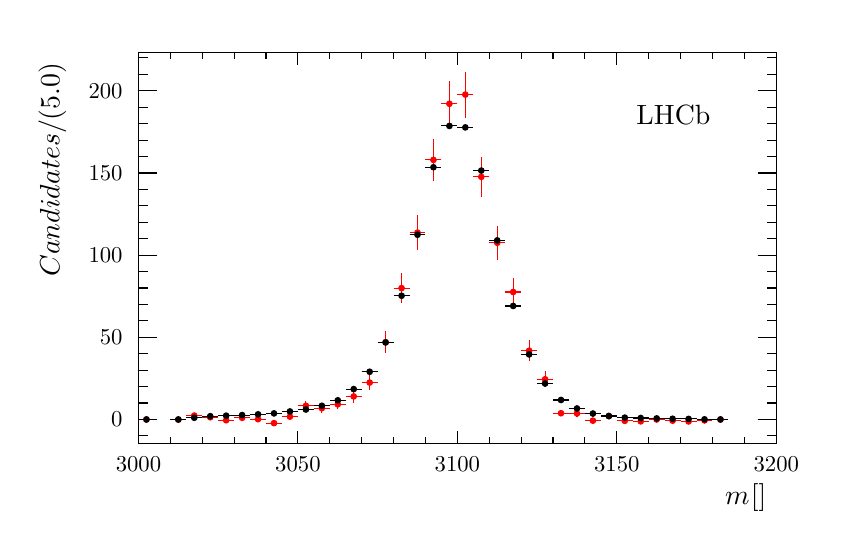
\begin{tikzpicture}
\pgfdeclareplotmark{cross} {
\pgfpathmoveto{\pgfpoint{-0.3\pgfplotmarksize}{\pgfplotmarksize}}
\pgfpathlineto{\pgfpoint{+0.3\pgfplotmarksize}{\pgfplotmarksize}}
\pgfpathlineto{\pgfpoint{+0.3\pgfplotmarksize}{0.3\pgfplotmarksize}}
\pgfpathlineto{\pgfpoint{+1\pgfplotmarksize}{0.3\pgfplotmarksize}}
\pgfpathlineto{\pgfpoint{+1\pgfplotmarksize}{-0.3\pgfplotmarksize}}
\pgfpathlineto{\pgfpoint{+0.3\pgfplotmarksize}{-0.3\pgfplotmarksize}}
\pgfpathlineto{\pgfpoint{+0.3\pgfplotmarksize}{-1.\pgfplotmarksize}}
\pgfpathlineto{\pgfpoint{-0.3\pgfplotmarksize}{-1.\pgfplotmarksize}}
\pgfpathlineto{\pgfpoint{-0.3\pgfplotmarksize}{-0.3\pgfplotmarksize}}
\pgfpathlineto{\pgfpoint{-1.\pgfplotmarksize}{-0.3\pgfplotmarksize}}
\pgfpathlineto{\pgfpoint{-1.\pgfplotmarksize}{0.3\pgfplotmarksize}}
\pgfpathlineto{\pgfpoint{-0.3\pgfplotmarksize}{0.3\pgfplotmarksize}}
\pgfpathclose
\pgfusepathqstroke
}
\pgfdeclareplotmark{cross*} {
\pgfpathmoveto{\pgfpoint{-0.3\pgfplotmarksize}{\pgfplotmarksize}}
\pgfpathlineto{\pgfpoint{+0.3\pgfplotmarksize}{\pgfplotmarksize}}
\pgfpathlineto{\pgfpoint{+0.3\pgfplotmarksize}{0.3\pgfplotmarksize}}
\pgfpathlineto{\pgfpoint{+1\pgfplotmarksize}{0.3\pgfplotmarksize}}
\pgfpathlineto{\pgfpoint{+1\pgfplotmarksize}{-0.3\pgfplotmarksize}}
\pgfpathlineto{\pgfpoint{+0.3\pgfplotmarksize}{-0.3\pgfplotmarksize}}
\pgfpathlineto{\pgfpoint{+0.3\pgfplotmarksize}{-1.\pgfplotmarksize}}
\pgfpathlineto{\pgfpoint{-0.3\pgfplotmarksize}{-1.\pgfplotmarksize}}
\pgfpathlineto{\pgfpoint{-0.3\pgfplotmarksize}{-0.3\pgfplotmarksize}}
\pgfpathlineto{\pgfpoint{-1.\pgfplotmarksize}{-0.3\pgfplotmarksize}}
\pgfpathlineto{\pgfpoint{-1.\pgfplotmarksize}{0.3\pgfplotmarksize}}
\pgfpathlineto{\pgfpoint{-0.3\pgfplotmarksize}{0.3\pgfplotmarksize}}
\pgfpathclose
\pgfusepathqfillstroke
}
\pgfdeclareplotmark{newstar} {
\pgfpathmoveto{\pgfqpoint{0pt}{\pgfplotmarksize}}
\pgfpathlineto{\pgfqpointpolar{44}{0.5\pgfplotmarksize}}
\pgfpathlineto{\pgfqpointpolar{18}{\pgfplotmarksize}}
\pgfpathlineto{\pgfqpointpolar{-20}{0.5\pgfplotmarksize}}
\pgfpathlineto{\pgfqpointpolar{-54}{\pgfplotmarksize}}
\pgfpathlineto{\pgfqpointpolar{-90}{0.5\pgfplotmarksize}}
\pgfpathlineto{\pgfqpointpolar{234}{\pgfplotmarksize}}
\pgfpathlineto{\pgfqpointpolar{198}{0.5\pgfplotmarksize}}
\pgfpathlineto{\pgfqpointpolar{162}{\pgfplotmarksize}}
\pgfpathlineto{\pgfqpointpolar{134}{0.5\pgfplotmarksize}}
\pgfpathclose
\pgfusepathqstroke
}
\pgfdeclareplotmark{newstar*} {
\pgfpathmoveto{\pgfqpoint{0pt}{\pgfplotmarksize}}
\pgfpathlineto{\pgfqpointpolar{44}{0.5\pgfplotmarksize}}
\pgfpathlineto{\pgfqpointpolar{18}{\pgfplotmarksize}}
\pgfpathlineto{\pgfqpointpolar{-20}{0.5\pgfplotmarksize}}
\pgfpathlineto{\pgfqpointpolar{-54}{\pgfplotmarksize}}
\pgfpathlineto{\pgfqpointpolar{-90}{0.5\pgfplotmarksize}}
\pgfpathlineto{\pgfqpointpolar{234}{\pgfplotmarksize}}
\pgfpathlineto{\pgfqpointpolar{198}{0.5\pgfplotmarksize}}
\pgfpathlineto{\pgfqpointpolar{162}{\pgfplotmarksize}}
\pgfpathlineto{\pgfqpointpolar{134}{0.5\pgfplotmarksize}}
\pgfpathclose
\pgfusepathqfillstroke
}
\definecolor{c}{rgb}{1,1,1};
\draw [color=c, fill=c] (0,0) rectangle (10,6.27517);
\draw [color=c, fill=c] (1.4,1.00403) rectangle (9.5,5.96141);
\definecolor{c}{rgb}{0,0,0};
\draw [c] (1.4,1.00403) -- (1.4,5.96141) -- (9.5,5.96141) -- (9.5,1.00403) -- (1.4,1.00403);
\definecolor{c}{rgb}{1,1,1};
\draw [color=c, fill=c] (1.4,1.00403) rectangle (9.5,5.96141);
\definecolor{c}{rgb}{0,0,0};
\draw [c] (1.4,1.00403) -- (1.4,5.96141) -- (9.5,5.96141) -- (9.5,1.00403) -- (1.4,1.00403);
\definecolor{c}{rgb}{1,0,0};
\draw [c,line width=0.4] (1.50125,1.30324) -- (1.50125,1.30603);
\draw [c,line width=0.4] (1.50125,1.30603) -- (1.50125,1.30881);
\draw [c,line width=0.4] (1.4,1.30603) -- (1.50125,1.30603);
\draw [c,line width=0.4] (1.50125,1.30603) -- (1.6025,1.30603);
\foreach \P in {(1.50125,1.30603)}{\draw[mark options={color=c,fill=c},mark size=2.402402pt,mark=*,mark size=1pt] plot coordinates {\P};}
\draw [c,line width=0.4] (1.90625,1.29671) -- (1.90625,1.30391);
\draw [c,line width=0.4] (1.90625,1.30391) -- (1.90625,1.31111);
\draw [c,line width=0.4] (1.805,1.30391) -- (1.90625,1.30391);
\draw [c,line width=0.4] (1.90625,1.30391) -- (2.0075,1.30391);
\foreach \P in {(1.90625,1.30391)}{\draw[mark options={color=c,fill=c},mark size=2.402402pt,mark=*,mark size=1pt] plot coordinates {\P};}
\draw [c,line width=0.4] (2.10875,1.32395) -- (2.10875,1.35619);
\draw [c,line width=0.4] (2.10875,1.35619) -- (2.10875,1.38842);
\draw [c,line width=0.4] (2.0075,1.35619) -- (2.10875,1.35619);
\draw [c,line width=0.4] (2.10875,1.35619) -- (2.21,1.35619);
\foreach \P in {(2.10875,1.35619)}{\draw[mark options={color=c,fill=c},mark size=2.402402pt,mark=*,mark size=1pt] plot coordinates {\P};}
\draw [c,line width=0.4] (2.31125,1.31018) -- (2.31125,1.33432);
\draw [c,line width=0.4] (2.31125,1.33432) -- (2.31125,1.35846);
\draw [c,line width=0.4] (2.21,1.33432) -- (2.31125,1.33432);
\draw [c,line width=0.4] (2.31125,1.33432) -- (2.4125,1.33432);
\foreach \P in {(2.31125,1.33432)}{\draw[mark options={color=c,fill=c},mark size=2.402402pt,mark=*,mark size=1pt] plot coordinates {\P};}
\draw [c,line width=0.4] (2.51375,1.28236) -- (2.51375,1.29663);
\draw [c,line width=0.4] (2.51375,1.29663) -- (2.51375,1.31091);
\draw [c,line width=0.4] (2.4125,1.29663) -- (2.51375,1.29663);
\draw [c,line width=0.4] (2.51375,1.29663) -- (2.615,1.29663);
\foreach \P in {(2.51375,1.29663)}{\draw[mark options={color=c,fill=c},mark size=2.402402pt,mark=*,mark size=1pt] plot coordinates {\P};}
\draw [c,line width=0.4] (2.71625,1.30645) -- (2.71625,1.32737);
\draw [c,line width=0.4] (2.71625,1.32737) -- (2.71625,1.3483);
\draw [c,line width=0.4] (2.615,1.32737) -- (2.71625,1.32737);
\draw [c,line width=0.4] (2.71625,1.32737) -- (2.8175,1.32737);
\foreach \P in {(2.71625,1.32737)}{\draw[mark options={color=c,fill=c},mark size=2.402402pt,mark=*,mark size=1pt] plot coordinates {\P};}
\draw [c,line width=0.4] (2.91875,1.30127) -- (2.91875,1.31034);
\draw [c,line width=0.4] (2.91875,1.31034) -- (2.91875,1.31942);
\draw [c,line width=0.4] (2.8175,1.31034) -- (2.91875,1.31034);
\draw [c,line width=0.4] (2.91875,1.31034) -- (3.02,1.31034);
\foreach \P in {(2.91875,1.31034)}{\draw[mark options={color=c,fill=c},mark size=2.402402pt,mark=*,mark size=1pt] plot coordinates {\P};}
\draw [c,line width=0.4] (3.12125,1.22885) -- (3.12125,1.25998);
\draw [c,line width=0.4] (3.12125,1.25998) -- (3.12125,1.2911);
\draw [c,line width=0.4] (3.02,1.25998) -- (3.12125,1.25998);
\draw [c,line width=0.4] (3.12125,1.25998) -- (3.2225,1.25998);
\foreach \P in {(3.12125,1.25998)}{\draw[mark options={color=c,fill=c},mark size=2.402402pt,mark=*,mark size=1pt] plot coordinates {\P};}
\draw [c,line width=0.4] (3.32375,1.31491) -- (3.32375,1.34227);
\draw [c,line width=0.4] (3.32375,1.34227) -- (3.32375,1.36964);
\draw [c,line width=0.4] (3.2225,1.34227) -- (3.32375,1.34227);
\draw [c,line width=0.4] (3.32375,1.34227) -- (3.425,1.34227);
\foreach \P in {(3.32375,1.34227)}{\draw[mark options={color=c,fill=c},mark size=2.402402pt,mark=*,mark size=1pt] plot coordinates {\P};}
\draw [c,line width=0.4] (3.52625,1.42021) -- (3.52625,1.48049);
\draw [c,line width=0.4] (3.52625,1.48049) -- (3.52625,1.54076);
\draw [c,line width=0.4] (3.425,1.48049) -- (3.52625,1.48049);
\draw [c,line width=0.4] (3.52625,1.48049) -- (3.6275,1.48049);
\foreach \P in {(3.52625,1.48049)}{\draw[mark options={color=c,fill=c},mark size=2.402402pt,mark=*,mark size=1pt] plot coordinates {\P};}
\draw [c,line width=0.4] (3.72875,1.39472) -- (3.72875,1.44933);
\draw [c,line width=0.4] (3.72875,1.44933) -- (3.72875,1.50395);
\draw [c,line width=0.4] (3.6275,1.44933) -- (3.72875,1.44933);
\draw [c,line width=0.4] (3.72875,1.44933) -- (3.83,1.44933);
\foreach \P in {(3.72875,1.44933)}{\draw[mark options={color=c,fill=c},mark size=2.402402pt,mark=*,mark size=1pt] plot coordinates {\P};}
\draw [c,line width=0.4] (3.93125,1.43522) -- (3.93125,1.49855);
\draw [c,line width=0.4] (3.93125,1.49855) -- (3.93125,1.56187);
\draw [c,line width=0.4] (3.83,1.49855) -- (3.93125,1.49855);
\draw [c,line width=0.4] (3.93125,1.49855) -- (4.0325,1.49855);
\foreach \P in {(3.93125,1.49855)}{\draw[mark options={color=c,fill=c},mark size=2.402402pt,mark=*,mark size=1pt] plot coordinates {\P};}
\draw [c,line width=0.4] (4.13375,1.52109) -- (4.13375,1.59927);
\draw [c,line width=0.4] (4.13375,1.59927) -- (4.13375,1.67745);
\draw [c,line width=0.4] (4.0325,1.59927) -- (4.13375,1.59927);
\draw [c,line width=0.4] (4.13375,1.59927) -- (4.235,1.59927);
\foreach \P in {(4.13375,1.59927)}{\draw[mark options={color=c,fill=c},mark size=2.402402pt,mark=*,mark size=1pt] plot coordinates {\P};}
\draw [c,line width=0.4] (4.33625,1.67614) -- (4.33625,1.77504);
\draw [c,line width=0.4] (4.33625,1.77504) -- (4.33625,1.87394);
\draw [c,line width=0.4] (4.235,1.77504) -- (4.33625,1.77504);
\draw [c,line width=0.4] (4.33625,1.77504) -- (4.4375,1.77504);
\foreach \P in {(4.33625,1.77504)}{\draw[mark options={color=c,fill=c},mark size=2.402402pt,mark=*,mark size=1pt] plot coordinates {\P};}
\draw [c,line width=0.4] (4.53875,2.14493) -- (4.53875,2.28806);
\draw [c,line width=0.4] (4.53875,2.28806) -- (4.53875,2.4312);
\draw [c,line width=0.4] (4.4375,2.28806) -- (4.53875,2.28806);
\draw [c,line width=0.4] (4.53875,2.28806) -- (4.64,2.28806);
\foreach \P in {(4.53875,2.28806)}{\draw[mark options={color=c,fill=c},mark size=2.402402pt,mark=*,mark size=1pt] plot coordinates {\P};}
\draw [c,line width=0.4] (4.74125,2.7878) -- (4.74125,2.97437);
\draw [c,line width=0.4] (4.74125,2.97437) -- (4.74125,3.16095);
\draw [c,line width=0.4] (4.64,2.97437) -- (4.74125,2.97437);
\draw [c,line width=0.4] (4.74125,2.97437) -- (4.8425,2.97437);
\foreach \P in {(4.74125,2.97437)}{\draw[mark options={color=c,fill=c},mark size=2.402402pt,mark=*,mark size=1pt] plot coordinates {\P};}
\draw [c,line width=0.4] (4.94375,3.4574) -- (4.94375,3.67997);
\draw [c,line width=0.4] (4.94375,3.67997) -- (4.94375,3.90254);
\draw [c,line width=0.4] (4.8425,3.67997) -- (4.94375,3.67997);
\draw [c,line width=0.4] (4.94375,3.67997) -- (5.045,3.67997);
\foreach \P in {(4.94375,3.67997)}{\draw[mark options={color=c,fill=c},mark size=2.402402pt,mark=*,mark size=1pt] plot coordinates {\P};}
\draw [c,line width=0.4] (5.14625,4.34062) -- (5.14625,4.60291);
\draw [c,line width=0.4] (5.14625,4.60291) -- (5.14625,4.8652);
\draw [c,line width=0.4] (5.045,4.60291) -- (5.14625,4.60291);
\draw [c,line width=0.4] (5.14625,4.60291) -- (5.2475,4.60291);
\foreach \P in {(5.14625,4.60291)}{\draw[mark options={color=c,fill=c},mark size=2.402402pt,mark=*,mark size=1pt] plot coordinates {\P};}
\draw [c,line width=0.4] (5.34875,5.02659) -- (5.34875,5.31586);
\draw [c,line width=0.4] (5.34875,5.31586) -- (5.34875,5.60513);
\draw [c,line width=0.4] (5.2475,5.31586) -- (5.34875,5.31586);
\draw [c,line width=0.4] (5.34875,5.31586) -- (5.45,5.31586);
\foreach \P in {(5.34875,5.31586)}{\draw[mark options={color=c,fill=c},mark size=2.402402pt,mark=*,mark size=1pt] plot coordinates {\P};}
\draw [c,line width=0.4] (5.55125,5.13849) -- (5.55125,5.43192);
\draw [c,line width=0.4] (5.55125,5.43192) -- (5.55125,5.72534);
\draw [c,line width=0.4] (5.45,5.43192) -- (5.55125,5.43192);
\draw [c,line width=0.4] (5.55125,5.43192) -- (5.6525,5.43192);
\foreach \P in {(5.55125,5.43192)}{\draw[mark options={color=c,fill=c},mark size=2.402402pt,mark=*,mark size=1pt] plot coordinates {\P};}
\draw [c,line width=0.4] (5.75375,4.13405) -- (5.75375,4.38763);
\draw [c,line width=0.4] (5.75375,4.38763) -- (5.75375,4.64121);
\draw [c,line width=0.4] (5.6525,4.38763) -- (5.75375,4.38763);
\draw [c,line width=0.4] (5.75375,4.38763) -- (5.855,4.38763);
\foreach \P in {(5.75375,4.38763)}{\draw[mark options={color=c,fill=c},mark size=2.402402pt,mark=*,mark size=1pt] plot coordinates {\P};}
\draw [c,line width=0.4] (5.95625,3.33328) -- (5.95625,3.54965);
\draw [c,line width=0.4] (5.95625,3.54965) -- (5.95625,3.76602);
\draw [c,line width=0.4] (5.855,3.54965) -- (5.95625,3.54965);
\draw [c,line width=0.4] (5.95625,3.54965) -- (6.0575,3.54965);
\foreach \P in {(5.95625,3.54965)}{\draw[mark options={color=c,fill=c},mark size=2.402402pt,mark=*,mark size=1pt] plot coordinates {\P};}
\draw [c,line width=0.4] (6.15875,2.74147) -- (6.15875,2.92528);
\draw [c,line width=0.4] (6.15875,2.92528) -- (6.15875,3.10909);
\draw [c,line width=0.4] (6.0575,2.92528) -- (6.15875,2.92528);
\draw [c,line width=0.4] (6.15875,2.92528) -- (6.26,2.92528);
\foreach \P in {(6.15875,2.92528)}{\draw[mark options={color=c,fill=c},mark size=2.402402pt,mark=*,mark size=1pt] plot coordinates {\P};}
\draw [c,line width=0.4] (6.36125,2.0449) -- (6.36125,2.17992);
\draw [c,line width=0.4] (6.36125,2.17992) -- (6.36125,2.31494);
\draw [c,line width=0.4] (6.26,2.17992) -- (6.36125,2.17992);
\draw [c,line width=0.4] (6.36125,2.17992) -- (6.4625,2.17992);
\foreach \P in {(6.36125,2.17992)}{\draw[mark options={color=c,fill=c},mark size=2.402402pt,mark=*,mark size=1pt] plot coordinates {\P};}
\draw [c,line width=0.4] (6.56375,1.71396) -- (6.56375,1.81721);
\draw [c,line width=0.4] (6.56375,1.81721) -- (6.56375,1.92046);
\draw [c,line width=0.4] (6.4625,1.81721) -- (6.56375,1.81721);
\draw [c,line width=0.4] (6.56375,1.81721) -- (6.665,1.81721);
\foreach \P in {(6.56375,1.81721)}{\draw[mark options={color=c,fill=c},mark size=2.402402pt,mark=*,mark size=1pt] plot coordinates {\P};}
\draw [c,line width=0.4] (6.76625,1.34524) -- (6.76625,1.38599);
\draw [c,line width=0.4] (6.76625,1.38599) -- (6.76625,1.42675);
\draw [c,line width=0.4] (6.665,1.38599) -- (6.76625,1.38599);
\draw [c,line width=0.4] (6.76625,1.38599) -- (6.8675,1.38599);
\foreach \P in {(6.76625,1.38599)}{\draw[mark options={color=c,fill=c},mark size=2.402402pt,mark=*,mark size=1pt] plot coordinates {\P};}
\draw [c,line width=0.4] (6.96875,1.34342) -- (6.96875,1.38354);
\draw [c,line width=0.4] (6.96875,1.38354) -- (6.96875,1.42367);
\draw [c,line width=0.4] (6.8675,1.38354) -- (6.96875,1.38354);
\draw [c,line width=0.4] (6.96875,1.38354) -- (7.07,1.38354);
\foreach \P in {(6.96875,1.38354)}{\draw[mark options={color=c,fill=c},mark size=2.402402pt,mark=*,mark size=1pt] plot coordinates {\P};}
\draw [c,line width=0.4] (7.17125,1.27302) -- (7.17125,1.29097);
\draw [c,line width=0.4] (7.17125,1.29097) -- (7.17125,1.30891);
\draw [c,line width=0.4] (7.07,1.29097) -- (7.17125,1.29097);
\draw [c,line width=0.4] (7.17125,1.29097) -- (7.2725,1.29097);
\foreach \P in {(7.17125,1.29097)}{\draw[mark options={color=c,fill=c},mark size=2.402402pt,mark=*,mark size=1pt] plot coordinates {\P};}
\draw [c,line width=0.4] (7.37375,1.3195) -- (7.37375,1.34948);
\draw [c,line width=0.4] (7.37375,1.34948) -- (7.37375,1.37947);
\draw [c,line width=0.4] (7.2725,1.34948) -- (7.37375,1.34948);
\draw [c,line width=0.4] (7.37375,1.34948) -- (7.475,1.34948);
\foreach \P in {(7.37375,1.34948)}{\draw[mark options={color=c,fill=c},mark size=2.402402pt,mark=*,mark size=1pt] plot coordinates {\P};}
\draw [c,line width=0.4] (7.57625,1.26959) -- (7.57625,1.28877);
\draw [c,line width=0.4] (7.57625,1.28877) -- (7.57625,1.30795);
\draw [c,line width=0.4] (7.475,1.28877) -- (7.57625,1.28877);
\draw [c,line width=0.4] (7.57625,1.28877) -- (7.6775,1.28877);
\foreach \P in {(7.57625,1.28877)}{\draw[mark options={color=c,fill=c},mark size=2.402402pt,mark=*,mark size=1pt] plot coordinates {\P};}
\draw [c,line width=0.4] (7.77875,1.25999) -- (7.77875,1.28238);
\draw [c,line width=0.4] (7.77875,1.28238) -- (7.77875,1.30477);
\draw [c,line width=0.4] (7.6775,1.28238) -- (7.77875,1.28238);
\draw [c,line width=0.4] (7.77875,1.28238) -- (7.88,1.28238);
\foreach \P in {(7.77875,1.28238)}{\draw[mark options={color=c,fill=c},mark size=2.402402pt,mark=*,mark size=1pt] plot coordinates {\P};}
\draw [c,line width=0.4] (7.98125,1.30374) -- (7.98125,1.30612);
\draw [c,line width=0.4] (7.98125,1.30612) -- (7.98125,1.30851);
\draw [c,line width=0.4] (7.88,1.30612) -- (7.98125,1.30612);
\draw [c,line width=0.4] (7.98125,1.30612) -- (8.0825,1.30612);
\foreach \P in {(7.98125,1.30612)}{\draw[mark options={color=c,fill=c},mark size=2.402402pt,mark=*,mark size=1pt] plot coordinates {\P};}
\draw [c,line width=0.4] (8.18375,1.27288) -- (8.18375,1.29088);
\draw [c,line width=0.4] (8.18375,1.29088) -- (8.18375,1.30887);
\draw [c,line width=0.4] (8.0825,1.29088) -- (8.18375,1.29088);
\draw [c,line width=0.4] (8.18375,1.29088) -- (8.285,1.29088);
\foreach \P in {(8.18375,1.29088)}{\draw[mark options={color=c,fill=c},mark size=2.402402pt,mark=*,mark size=1pt] plot coordinates {\P};}
\draw [c,line width=0.4] (8.38625,1.25818) -- (8.38625,1.28114);
\draw [c,line width=0.4] (8.38625,1.28114) -- (8.38625,1.3041);
\draw [c,line width=0.4] (8.285,1.28114) -- (8.38625,1.28114);
\draw [c,line width=0.4] (8.38625,1.28114) -- (8.4875,1.28114);
\foreach \P in {(8.38625,1.28114)}{\draw[mark options={color=c,fill=c},mark size=2.402402pt,mark=*,mark size=1pt] plot coordinates {\P};}
\draw [c,line width=0.4] (8.58875,1.2789) -- (8.58875,1.29459);
\draw [c,line width=0.4] (8.58875,1.29459) -- (8.58875,1.31029);
\draw [c,line width=0.4] (8.4875,1.29459) -- (8.58875,1.29459);
\draw [c,line width=0.4] (8.58875,1.29459) -- (8.69,1.29459);
\foreach \P in {(8.58875,1.29459)}{\draw[mark options={color=c,fill=c},mark size=2.402402pt,mark=*,mark size=1pt] plot coordinates {\P};}
\draw [c,line width=0.4] (8.79125,1.30573) -- (8.79125,1.30642);
\draw [c,line width=0.4] (8.79125,1.30642) -- (8.79125,1.3071);
\draw [c,line width=0.4] (8.69,1.30642) -- (8.79125,1.30642);
\draw [c,line width=0.4] (8.79125,1.30642) -- (8.8925,1.30642);
\foreach \P in {(8.79125,1.30642)}{\draw[mark options={color=c,fill=c},mark size=2.402402pt,mark=*,mark size=1pt] plot coordinates {\P};}
\definecolor{c}{rgb}{0,0,0};
\draw [c,line width=0.4] (1.4,1.00403) -- (9.5,1.00403);
\draw [anchor= east] (9.5,0.317272) node[scale=1.00614, rotate=0]{$m_{\Jpsi} [\mevcc]$};
\draw [c,line width=0.4] (1.4,1.15651) -- (1.4,1.00403);
\draw [c,line width=0.4] (1.805,1.08027) -- (1.805,1.00403);
\draw [c,line width=0.4] (2.21,1.08027) -- (2.21,1.00403);
\draw [c,line width=0.4] (2.615,1.08027) -- (2.615,1.00403);
\draw [c,line width=0.4] (3.02,1.08027) -- (3.02,1.00403);
\draw [c,line width=0.4] (3.425,1.15651) -- (3.425,1.00403);
\draw [c,line width=0.4] (3.83,1.08027) -- (3.83,1.00403);
\draw [c,line width=0.4] (4.235,1.08027) -- (4.235,1.00403);
\draw [c,line width=0.4] (4.64,1.08027) -- (4.64,1.00403);
\draw [c,line width=0.4] (5.045,1.08027) -- (5.045,1.00403);
\draw [c,line width=0.4] (5.45,1.15651) -- (5.45,1.00403);
\draw [c,line width=0.4] (5.855,1.08027) -- (5.855,1.00403);
\draw [c,line width=0.4] (6.26,1.08027) -- (6.26,1.00403);
\draw [c,line width=0.4] (6.665,1.08027) -- (6.665,1.00403);
\draw [c,line width=0.4] (7.07,1.08027) -- (7.07,1.00403);
\draw [c,line width=0.4] (7.475,1.15651) -- (7.475,1.00403);
\draw [c,line width=0.4] (7.88,1.08027) -- (7.88,1.00403);
\draw [c,line width=0.4] (8.285,1.08027) -- (8.285,1.00403);
\draw [c,line width=0.4] (8.69,1.08027) -- (8.69,1.00403);
\draw [c,line width=0.4] (9.095,1.08027) -- (9.095,1.00403);
\draw [c,line width=0.4] (9.5,1.15651) -- (9.5,1.00403);
\draw [anchor=base] (1.4,0.640067) node[scale=0.819821, rotate=0]{3000};
\draw [anchor=base] (3.425,0.640067) node[scale=0.819821, rotate=0]{3050};
\draw [anchor=base] (5.45,0.640067) node[scale=0.819821, rotate=0]{3100};
\draw [anchor=base] (7.475,0.640067) node[scale=0.819821, rotate=0]{3150};
\draw [anchor=base] (9.5,0.640067) node[scale=0.819821, rotate=0]{3200};
\draw [c,line width=0.4] (1.4,5.96141) -- (9.5,5.96141);
\draw [c,line width=0.4] (1.4,5.80892) -- (1.4,5.96141);
\draw [c,line width=0.4] (1.805,5.88517) -- (1.805,5.96141);
\draw [c,line width=0.4] (2.21,5.88517) -- (2.21,5.96141);
\draw [c,line width=0.4] (2.615,5.88517) -- (2.615,5.96141);
\draw [c,line width=0.4] (3.02,5.88517) -- (3.02,5.96141);
\draw [c,line width=0.4] (3.425,5.80892) -- (3.425,5.96141);
\draw [c,line width=0.4] (3.83,5.88517) -- (3.83,5.96141);
\draw [c,line width=0.4] (4.235,5.88517) -- (4.235,5.96141);
\draw [c,line width=0.4] (4.64,5.88517) -- (4.64,5.96141);
\draw [c,line width=0.4] (5.045,5.88517) -- (5.045,5.96141);
\draw [c,line width=0.4] (5.45,5.80892) -- (5.45,5.96141);
\draw [c,line width=0.4] (5.855,5.88517) -- (5.855,5.96141);
\draw [c,line width=0.4] (6.26,5.88517) -- (6.26,5.96141);
\draw [c,line width=0.4] (6.665,5.88517) -- (6.665,5.96141);
\draw [c,line width=0.4] (7.07,5.88517) -- (7.07,5.96141);
\draw [c,line width=0.4] (7.475,5.80892) -- (7.475,5.96141);
\draw [c,line width=0.4] (7.88,5.88517) -- (7.88,5.96141);
\draw [c,line width=0.4] (8.285,5.88517) -- (8.285,5.96141);
\draw [c,line width=0.4] (8.69,5.88517) -- (8.69,5.96141);
\draw [c,line width=0.4] (9.095,5.88517) -- (9.095,5.96141);
\draw [c,line width=0.4] (9.5,5.80892) -- (9.5,5.96141);
\draw [c,line width=0.4] (1.4,1.00403) -- (1.4,5.96141);
\draw [anchor= east] (0.3056,5.96141) node[scale=1.00614, rotate=90]{$\text{Candidates} / (5.0 \mevcc)$};
\draw [c,line width=0.4] (1.637,1.3064) -- (1.4,1.3064);
\draw [c,line width=0.4] (1.5185,1.51509) -- (1.4,1.51509);
\draw [c,line width=0.4] (1.5185,1.72379) -- (1.4,1.72379);
\draw [c,line width=0.4] (1.5185,1.93249) -- (1.4,1.93249);
\draw [c,line width=0.4] (1.5185,2.14119) -- (1.4,2.14119);
\draw [c,line width=0.4] (1.637,2.34989) -- (1.4,2.34989);
\draw [c,line width=0.4] (1.5185,2.55858) -- (1.4,2.55858);
\draw [c,line width=0.4] (1.5185,2.76728) -- (1.4,2.76728);
\draw [c,line width=0.4] (1.5185,2.97598) -- (1.4,2.97598);
\draw [c,line width=0.4] (1.5185,3.18468) -- (1.4,3.18468);
\draw [c,line width=0.4] (1.637,3.39338) -- (1.4,3.39338);
\draw [c,line width=0.4] (1.5185,3.60207) -- (1.4,3.60207);
\draw [c,line width=0.4] (1.5185,3.81077) -- (1.4,3.81077);
\draw [c,line width=0.4] (1.5185,4.01947) -- (1.4,4.01947);
\draw [c,line width=0.4] (1.5185,4.22817) -- (1.4,4.22817);
\draw [c,line width=0.4] (1.637,4.43687) -- (1.4,4.43687);
\draw [c,line width=0.4] (1.5185,4.64556) -- (1.4,4.64556);
\draw [c,line width=0.4] (1.5185,4.85426) -- (1.4,4.85426);
\draw [c,line width=0.4] (1.5185,5.06296) -- (1.4,5.06296);
\draw [c,line width=0.4] (1.5185,5.27166) -- (1.4,5.27166);
\draw [c,line width=0.4] (1.637,5.48036) -- (1.4,5.48036);
\draw [c,line width=0.4] (1.637,1.3064) -- (1.4,1.3064);
\draw [c,line width=0.4] (1.5185,1.0977) -- (1.4,1.0977);
\draw [c,line width=0.4] (1.637,5.48036) -- (1.4,5.48036);
\draw [c,line width=0.4] (1.5185,5.68905) -- (1.4,5.68905);
\draw [c,line width=0.4] (1.5185,5.89775) -- (1.4,5.89775);
\draw [anchor= east] (1.3,1.3064) node[scale=0.819821, rotate=0]{0};
\draw [anchor= east] (1.3,2.34989) node[scale=0.819821, rotate=0]{50};
\draw [anchor= east] (1.3,3.39338) node[scale=0.819821, rotate=0]{100};
\draw [anchor= east] (1.3,4.43687) node[scale=0.819821, rotate=0]{150};
\draw [anchor= east] (1.3,5.48036) node[scale=0.819821, rotate=0]{200};
\draw [c,line width=0.4] (9.5,1.00403) -- (9.5,5.96141);
\draw [c,line width=0.4] (9.263,1.3064) -- (9.5,1.3064);
\draw [c,line width=0.4] (9.3815,1.51509) -- (9.5,1.51509);
\draw [c,line width=0.4] (9.3815,1.72379) -- (9.5,1.72379);
\draw [c,line width=0.4] (9.3815,1.93249) -- (9.5,1.93249);
\draw [c,line width=0.4] (9.3815,2.14119) -- (9.5,2.14119);
\draw [c,line width=0.4] (9.263,2.34989) -- (9.5,2.34989);
\draw [c,line width=0.4] (9.3815,2.55858) -- (9.5,2.55858);
\draw [c,line width=0.4] (9.3815,2.76728) -- (9.5,2.76728);
\draw [c,line width=0.4] (9.3815,2.97598) -- (9.5,2.97598);
\draw [c,line width=0.4] (9.3815,3.18468) -- (9.5,3.18468);
\draw [c,line width=0.4] (9.263,3.39338) -- (9.5,3.39338);
\draw [c,line width=0.4] (9.3815,3.60207) -- (9.5,3.60207);
\draw [c,line width=0.4] (9.3815,3.81077) -- (9.5,3.81077);
\draw [c,line width=0.4] (9.3815,4.01947) -- (9.5,4.01947);
\draw [c,line width=0.4] (9.3815,4.22817) -- (9.5,4.22817);
\draw [c,line width=0.4] (9.263,4.43687) -- (9.5,4.43687);
\draw [c,line width=0.4] (9.3815,4.64556) -- (9.5,4.64556);
\draw [c,line width=0.4] (9.3815,4.85426) -- (9.5,4.85426);
\draw [c,line width=0.4] (9.3815,5.06296) -- (9.5,5.06296);
\draw [c,line width=0.4] (9.3815,5.27166) -- (9.5,5.27166);
\draw [c,line width=0.4] (9.263,5.48036) -- (9.5,5.48036);
\draw [c,line width=0.4] (9.263,1.3064) -- (9.5,1.3064);
\draw [c,line width=0.4] (9.3815,1.0977) -- (9.5,1.0977);
\draw [c,line width=0.4] (9.263,5.48036) -- (9.5,5.48036);
\draw [c,line width=0.4] (9.3815,5.68905) -- (9.5,5.68905);
\draw [c,line width=0.4] (9.3815,5.89775) -- (9.5,5.89775);
\draw [c,line width=0.4] (1.50125,1.30639) -- (1.50125,1.3065);
\draw [c,line width=0.4] (1.50125,1.3065) -- (1.50125,1.30662);
\draw [c,line width=0.4] (1.4,1.3065) -- (1.50125,1.3065);
\draw [c,line width=0.4] (1.50125,1.3065) -- (1.6025,1.3065);
\foreach \P in {(1.50125,1.3065)}{\draw[mark options={color=c,fill=c},mark size=2.402402pt,mark=*,mark size=1pt] plot coordinates {\P};}
\draw [c,line width=0.4] (1.90625,1.30654) -- (1.90625,1.30676);
\draw [c,line width=0.4] (1.90625,1.30676) -- (1.90625,1.30698);
\draw [c,line width=0.4] (1.805,1.30676) -- (1.90625,1.30676);
\draw [c,line width=0.4] (1.90625,1.30676) -- (2.0075,1.30676);
\foreach \P in {(1.90625,1.30676)}{\draw[mark options={color=c,fill=c},mark size=2.402402pt,mark=*,mark size=1pt] plot coordinates {\P};}
\draw [c,line width=0.4] (2.10875,1.32621) -- (2.10875,1.32789);
\draw [c,line width=0.4] (2.10875,1.32789) -- (2.10875,1.32956);
\draw [c,line width=0.4] (2.0075,1.32789) -- (2.10875,1.32789);
\draw [c,line width=0.4] (2.10875,1.32789) -- (2.21,1.32789);
\foreach \P in {(2.10875,1.32789)}{\draw[mark options={color=c,fill=c},mark size=2.402402pt,mark=*,mark size=1pt] plot coordinates {\P};}
\draw [c,line width=0.4] (2.31125,1.34596) -- (2.31125,1.3483);
\draw [c,line width=0.4] (2.31125,1.3483) -- (2.31125,1.35064);
\draw [c,line width=0.4] (2.21,1.3483) -- (2.31125,1.3483);
\draw [c,line width=0.4] (2.31125,1.3483) -- (2.4125,1.3483);
\foreach \P in {(2.31125,1.3483)}{\draw[mark options={color=c,fill=c},mark size=2.402402pt,mark=*,mark size=1pt] plot coordinates {\P};}
\draw [c,line width=0.4] (2.51375,1.35205) -- (2.51375,1.35455);
\draw [c,line width=0.4] (2.51375,1.35455) -- (2.51375,1.35706);
\draw [c,line width=0.4] (2.4125,1.35455) -- (2.51375,1.35455);
\draw [c,line width=0.4] (2.51375,1.35455) -- (2.615,1.35455);
\foreach \P in {(2.51375,1.35455)}{\draw[mark options={color=c,fill=c},mark size=2.402402pt,mark=*,mark size=1pt] plot coordinates {\P};}
\draw [c,line width=0.4] (2.71625,1.35948) -- (2.71625,1.36218);
\draw [c,line width=0.4] (2.71625,1.36218) -- (2.71625,1.36487);
\draw [c,line width=0.4] (2.615,1.36218) -- (2.71625,1.36218);
\draw [c,line width=0.4] (2.71625,1.36218) -- (2.8175,1.36218);
\foreach \P in {(2.71625,1.36218)}{\draw[mark options={color=c,fill=c},mark size=2.402402pt,mark=*,mark size=1pt] plot coordinates {\P};}
\draw [c,line width=0.4] (2.91875,1.36863) -- (2.91875,1.37154);
\draw [c,line width=0.4] (2.91875,1.37154) -- (2.91875,1.37445);
\draw [c,line width=0.4] (2.8175,1.37154) -- (2.91875,1.37154);
\draw [c,line width=0.4] (2.91875,1.37154) -- (3.02,1.37154);
\foreach \P in {(2.91875,1.37154)}{\draw[mark options={color=c,fill=c},mark size=2.402402pt,mark=*,mark size=1pt] plot coordinates {\P};}
\draw [c,line width=0.4] (3.12125,1.38049) -- (3.12125,1.38366);
\draw [c,line width=0.4] (3.12125,1.38366) -- (3.12125,1.38683);
\draw [c,line width=0.4] (3.02,1.38366) -- (3.12125,1.38366);
\draw [c,line width=0.4] (3.12125,1.38366) -- (3.2225,1.38366);
\foreach \P in {(3.12125,1.38366)}{\draw[mark options={color=c,fill=c},mark size=2.402402pt,mark=*,mark size=1pt] plot coordinates {\P};}
\draw [c,line width=0.4] (3.32375,1.40476) -- (3.32375,1.4084);
\draw [c,line width=0.4] (3.32375,1.4084) -- (3.32375,1.41204);
\draw [c,line width=0.4] (3.2225,1.4084) -- (3.32375,1.4084);
\draw [c,line width=0.4] (3.32375,1.4084) -- (3.425,1.4084);
\foreach \P in {(3.32375,1.4084)}{\draw[mark options={color=c,fill=c},mark size=2.402402pt,mark=*,mark size=1pt] plot coordinates {\P};}
\draw [c,line width=0.4] (3.52625,1.42853) -- (3.52625,1.43258);
\draw [c,line width=0.4] (3.52625,1.43258) -- (3.52625,1.43663);
\draw [c,line width=0.4] (3.425,1.43258) -- (3.52625,1.43258);
\draw [c,line width=0.4] (3.52625,1.43258) -- (3.6275,1.43258);
\foreach \P in {(3.52625,1.43258)}{\draw[mark options={color=c,fill=c},mark size=2.402402pt,mark=*,mark size=1pt] plot coordinates {\P};}
\draw [c,line width=0.4] (3.72875,1.47545) -- (3.72875,1.4802);
\draw [c,line width=0.4] (3.72875,1.4802) -- (3.72875,1.48496);
\draw [c,line width=0.4] (3.6275,1.4802) -- (3.72875,1.4802);
\draw [c,line width=0.4] (3.72875,1.4802) -- (3.83,1.4802);
\foreach \P in {(3.72875,1.4802)}{\draw[mark options={color=c,fill=c},mark size=2.402402pt,mark=*,mark size=1pt] plot coordinates {\P};}
\draw [c,line width=0.4] (3.93125,1.54425) -- (3.93125,1.54988);
\draw [c,line width=0.4] (3.93125,1.54988) -- (3.93125,1.55551);
\draw [c,line width=0.4] (3.83,1.54988) -- (3.93125,1.54988);
\draw [c,line width=0.4] (3.93125,1.54988) -- (4.0325,1.54988);
\foreach \P in {(3.93125,1.54988)}{\draw[mark options={color=c,fill=c},mark size=2.402402pt,mark=*,mark size=1pt] plot coordinates {\P};}
\draw [c,line width=0.4] (4.13375,1.68503) -- (4.13375,1.69211);
\draw [c,line width=0.4] (4.13375,1.69211) -- (4.13375,1.6992);
\draw [c,line width=0.4] (4.0325,1.69211) -- (4.13375,1.69211);
\draw [c,line width=0.4] (4.13375,1.69211) -- (4.235,1.69211);
\foreach \P in {(4.13375,1.69211)}{\draw[mark options={color=c,fill=c},mark size=2.402402pt,mark=*,mark size=1pt] plot coordinates {\P};}
\draw [c,line width=0.4] (4.33625,1.90343) -- (4.33625,1.91232);
\draw [c,line width=0.4] (4.33625,1.91232) -- (4.33625,1.9212);
\draw [c,line width=0.4] (4.235,1.91232) -- (4.33625,1.91232);
\draw [c,line width=0.4] (4.33625,1.91232) -- (4.4375,1.91232);
\foreach \P in {(4.33625,1.91232)}{\draw[mark options={color=c,fill=c},mark size=2.402402pt,mark=*,mark size=1pt] plot coordinates {\P};}
\draw [c,line width=0.4] (4.53875,2.27322) -- (4.53875,2.2845);
\draw [c,line width=0.4] (4.53875,2.2845) -- (4.53875,2.29579);
\draw [c,line width=0.4] (4.4375,2.2845) -- (4.53875,2.2845);
\draw [c,line width=0.4] (4.53875,2.2845) -- (4.64,2.2845);
\foreach \P in {(4.53875,2.2845)}{\draw[mark options={color=c,fill=c},mark size=2.402402pt,mark=*,mark size=1pt] plot coordinates {\P};}
\draw [c,line width=0.4] (4.74125,2.86351) -- (4.74125,2.87781);
\draw [c,line width=0.4] (4.74125,2.87781) -- (4.74125,2.89212);
\draw [c,line width=0.4] (4.64,2.87781) -- (4.74125,2.87781);
\draw [c,line width=0.4] (4.74125,2.87781) -- (4.8425,2.87781);
\foreach \P in {(4.74125,2.87781)}{\draw[mark options={color=c,fill=c},mark size=2.402402pt,mark=*,mark size=1pt] plot coordinates {\P};}
\draw [c,line width=0.4] (4.94375,3.63495) -- (4.94375,3.65242);
\draw [c,line width=0.4] (4.94375,3.65242) -- (4.94375,3.6699);
\draw [c,line width=0.4] (4.8425,3.65242) -- (4.94375,3.65242);
\draw [c,line width=0.4] (4.94375,3.65242) -- (5.045,3.65242);
\foreach \P in {(4.94375,3.65242)}{\draw[mark options={color=c,fill=c},mark size=2.402402pt,mark=*,mark size=1pt] plot coordinates {\P};}
\draw [c,line width=0.4] (5.14625,4.48903) -- (5.14625,4.50945);
\draw [c,line width=0.4] (5.14625,4.50945) -- (5.14625,4.52987);
\draw [c,line width=0.4] (5.045,4.50945) -- (5.14625,4.50945);
\draw [c,line width=0.4] (5.14625,4.50945) -- (5.2475,4.50945);
\foreach \P in {(5.14625,4.50945)}{\draw[mark options={color=c,fill=c},mark size=2.402402pt,mark=*,mark size=1pt] plot coordinates {\P};}
\draw [c,line width=0.4] (5.34875,5.01218) -- (5.34875,5.0342);
\draw [c,line width=0.4] (5.34875,5.0342) -- (5.34875,5.05623);
\draw [c,line width=0.4] (5.2475,5.0342) -- (5.34875,5.0342);
\draw [c,line width=0.4] (5.34875,5.0342) -- (5.45,5.0342);
\foreach \P in {(5.34875,5.0342)}{\draw[mark options={color=c,fill=c},mark size=2.402402pt,mark=*,mark size=1pt] plot coordinates {\P};}
\draw [c,line width=0.4] (5.55125,4.99376) -- (5.55125,5.01573);
\draw [c,line width=0.4] (5.55125,5.01573) -- (5.55125,5.03771);
\draw [c,line width=0.4] (5.45,5.01573) -- (5.55125,5.01573);
\draw [c,line width=0.4] (5.55125,5.01573) -- (5.6525,5.01573);
\foreach \P in {(5.55125,5.01573)}{\draw[mark options={color=c,fill=c},mark size=2.402402pt,mark=*,mark size=1pt] plot coordinates {\P};}
\draw [c,line width=0.4] (5.75375,4.44727) -- (5.75375,4.46756);
\draw [c,line width=0.4] (5.75375,4.46756) -- (5.75375,4.48784);
\draw [c,line width=0.4] (5.6525,4.46756) -- (5.75375,4.46756);
\draw [c,line width=0.4] (5.75375,4.46756) -- (5.855,4.46756);
\foreach \P in {(5.75375,4.46756)}{\draw[mark options={color=c,fill=c},mark size=2.402402pt,mark=*,mark size=1pt] plot coordinates {\P};}
\draw [c,line width=0.4] (5.95625,3.56369) -- (5.95625,3.5809);
\draw [c,line width=0.4] (5.95625,3.5809) -- (5.95625,3.5981);
\draw [c,line width=0.4] (5.855,3.5809) -- (5.95625,3.5809);
\draw [c,line width=0.4] (5.95625,3.5809) -- (6.0575,3.5809);
\foreach \P in {(5.95625,3.5809)}{\draw[mark options={color=c,fill=c},mark size=2.402402pt,mark=*,mark size=1pt] plot coordinates {\P};}
\draw [c,line width=0.4] (6.15875,2.7343) -- (6.15875,2.748);
\draw [c,line width=0.4] (6.15875,2.748) -- (6.15875,2.7617);
\draw [c,line width=0.4] (6.0575,2.748) -- (6.15875,2.748);
\draw [c,line width=0.4] (6.15875,2.748) -- (6.26,2.748);
\foreach \P in {(6.15875,2.748)}{\draw[mark options={color=c,fill=c},mark size=2.402402pt,mark=*,mark size=1pt] plot coordinates {\P};}
\draw [c,line width=0.4] (6.36125,2.12243) -- (6.36125,2.1328);
\draw [c,line width=0.4] (6.36125,2.1328) -- (6.36125,2.14318);
\draw [c,line width=0.4] (6.26,2.1328) -- (6.36125,2.1328);
\draw [c,line width=0.4] (6.36125,2.1328) -- (6.4625,2.1328);
\foreach \P in {(6.36125,2.1328)}{\draw[mark options={color=c,fill=c},mark size=2.402402pt,mark=*,mark size=1pt] plot coordinates {\P};}
\draw [c,line width=0.4] (6.56375,1.75512) -- (6.56375,1.76283);
\draw [c,line width=0.4] (6.56375,1.76283) -- (6.56375,1.77054);
\draw [c,line width=0.4] (6.4625,1.76283) -- (6.56375,1.76283);
\draw [c,line width=0.4] (6.56375,1.76283) -- (6.665,1.76283);
\foreach \P in {(6.56375,1.76283)}{\draw[mark options={color=c,fill=c},mark size=2.402402pt,mark=*,mark size=1pt] plot coordinates {\P};}
\draw [c,line width=0.4] (6.76625,1.54821) -- (6.76625,1.55389);
\draw [c,line width=0.4] (6.76625,1.55389) -- (6.76625,1.55957);
\draw [c,line width=0.4] (6.665,1.55389) -- (6.76625,1.55389);
\draw [c,line width=0.4] (6.76625,1.55389) -- (6.8675,1.55389);
\foreach \P in {(6.76625,1.55389)}{\draw[mark options={color=c,fill=c},mark size=2.402402pt,mark=*,mark size=1pt] plot coordinates {\P};}
\draw [c,line width=0.4] (6.96875,1.44177) -- (6.96875,1.44604);
\draw [c,line width=0.4] (6.96875,1.44604) -- (6.96875,1.4503);
\draw [c,line width=0.4] (6.8675,1.44604) -- (6.96875,1.44604);
\draw [c,line width=0.4] (6.96875,1.44604) -- (7.07,1.44604);
\foreach \P in {(6.96875,1.44604)}{\draw[mark options={color=c,fill=c},mark size=2.402402pt,mark=*,mark size=1pt] plot coordinates {\P};}
\draw [c,line width=0.4] (7.17125,1.37839) -- (7.17125,1.38152);
\draw [c,line width=0.4] (7.17125,1.38152) -- (7.17125,1.38464);
\draw [c,line width=0.4] (7.07,1.38152) -- (7.17125,1.38152);
\draw [c,line width=0.4] (7.17125,1.38152) -- (7.2725,1.38152);
\foreach \P in {(7.17125,1.38152)}{\draw[mark options={color=c,fill=c},mark size=2.402402pt,mark=*,mark size=1pt] plot coordinates {\P};}
\draw [c,line width=0.4] (7.37375,1.34742) -- (7.37375,1.34979);
\draw [c,line width=0.4] (7.37375,1.34979) -- (7.37375,1.35217);
\draw [c,line width=0.4] (7.2725,1.34979) -- (7.37375,1.34979);
\draw [c,line width=0.4] (7.37375,1.34979) -- (7.475,1.34979);
\foreach \P in {(7.37375,1.34979)}{\draw[mark options={color=c,fill=c},mark size=2.402402pt,mark=*,mark size=1pt] plot coordinates {\P};}
\draw [c,line width=0.4] (7.57625,1.3281) -- (7.57625,1.32984);
\draw [c,line width=0.4] (7.57625,1.32984) -- (7.57625,1.33159);
\draw [c,line width=0.4] (7.475,1.32984) -- (7.57625,1.32984);
\draw [c,line width=0.4] (7.57625,1.32984) -- (7.6775,1.32984);
\foreach \P in {(7.57625,1.32984)}{\draw[mark options={color=c,fill=c},mark size=2.402402pt,mark=*,mark size=1pt] plot coordinates {\P};}
\draw [c,line width=0.4] (7.77875,1.32347) -- (7.77875,1.32503);
\draw [c,line width=0.4] (7.77875,1.32503) -- (7.77875,1.32659);
\draw [c,line width=0.4] (7.6775,1.32503) -- (7.77875,1.32503);
\draw [c,line width=0.4] (7.77875,1.32503) -- (7.88,1.32503);
\foreach \P in {(7.77875,1.32503)}{\draw[mark options={color=c,fill=c},mark size=2.402402pt,mark=*,mark size=1pt] plot coordinates {\P};}
\draw [c,line width=0.4] (7.98125,1.31872) -- (7.98125,1.32005);
\draw [c,line width=0.4] (7.98125,1.32005) -- (7.98125,1.32139);
\draw [c,line width=0.4] (7.88,1.32005) -- (7.98125,1.32005);
\draw [c,line width=0.4] (7.98125,1.32005) -- (8.0825,1.32005);
\foreach \P in {(7.98125,1.32005)}{\draw[mark options={color=c,fill=c},mark size=2.402402pt,mark=*,mark size=1pt] plot coordinates {\P};}
\draw [c,line width=0.4] (8.18375,1.31423) -- (8.18375,1.31531);
\draw [c,line width=0.4] (8.18375,1.31531) -- (8.18375,1.31639);
\draw [c,line width=0.4] (8.0825,1.31531) -- (8.18375,1.31531);
\draw [c,line width=0.4] (8.18375,1.31531) -- (8.285,1.31531);
\foreach \P in {(8.18375,1.31531)}{\draw[mark options={color=c,fill=c},mark size=2.402402pt,mark=*,mark size=1pt] plot coordinates {\P};}
\draw [c,line width=0.4] (8.38625,1.31259) -- (8.38625,1.31356);
\draw [c,line width=0.4] (8.38625,1.31356) -- (8.38625,1.31452);
\draw [c,line width=0.4] (8.285,1.31356) -- (8.38625,1.31356);
\draw [c,line width=0.4] (8.38625,1.31356) -- (8.4875,1.31356);
\foreach \P in {(8.38625,1.31356)}{\draw[mark options={color=c,fill=c},mark size=2.402402pt,mark=*,mark size=1pt] plot coordinates {\P};}
\draw [c,line width=0.4] (8.58875,1.30768) -- (8.58875,1.30816);
\draw [c,line width=0.4] (8.58875,1.30816) -- (8.58875,1.30863);
\draw [c,line width=0.4] (8.4875,1.30816) -- (8.58875,1.30816);
\draw [c,line width=0.4] (8.58875,1.30816) -- (8.69,1.30816);
\foreach \P in {(8.58875,1.30816)}{\draw[mark options={color=c,fill=c},mark size=2.402402pt,mark=*,mark size=1pt] plot coordinates {\P};}
\draw [c,line width=0.4] (8.79125,1.3064) -- (8.79125,1.30653);
\draw [c,line width=0.4] (8.79125,1.30653) -- (8.79125,1.30666);
\draw [c,line width=0.4] (8.69,1.30653) -- (8.79125,1.30653);
\draw [c,line width=0.4] (8.79125,1.30653) -- (8.8925,1.30653);
\foreach \P in {(8.79125,1.30653)}{\draw[mark options={color=c,fill=c},mark size=2.402402pt,mark=*,mark size=1pt] plot coordinates {\P};}
\draw [anchor= west] (7.6,5.17701) node[scale=1.00614, rotate=0]{LHCb};
\end{tikzpicture}
